\documentclass[tikz,border=2pt]{standalone}
\usetikzlibrary{calc}
\usetikzlibrary{intersections}
\usetikzlibrary{patterns}
\usepackage{bm}
\usetikzlibrary{positioning}
\usetikzlibrary{shapes}
\usepackage{pgfplots}
\pgfplotsset{compat=1.18}

\begin{document}

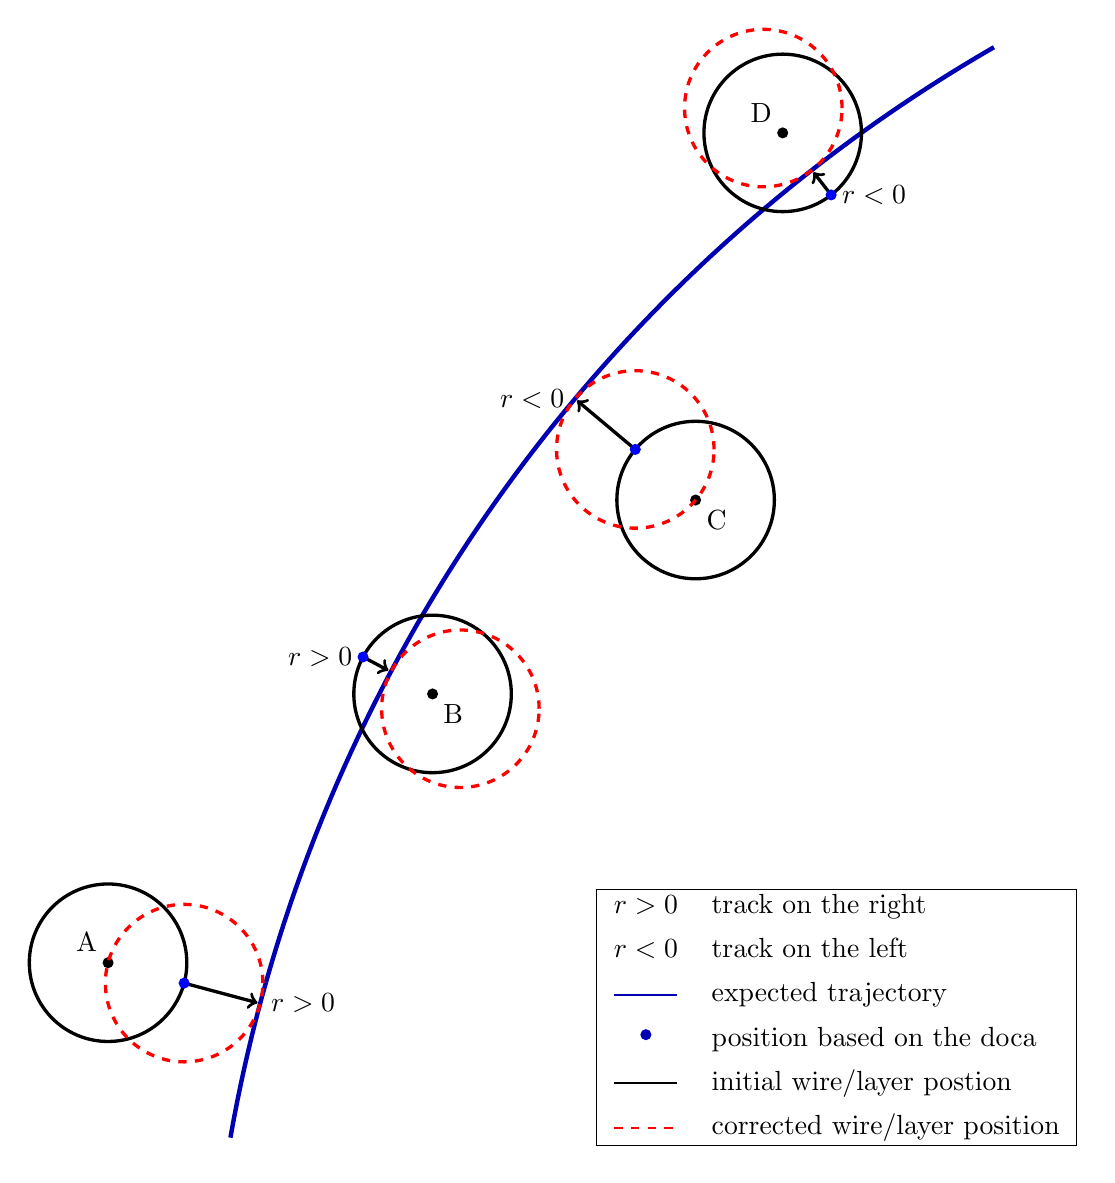
\begin{tikzpicture}[very thick]
    % \tikzset{
    %     every node/.style={font=\scriptsize}
    % }
    
    % ---- Notes ----
    % Track : portion of circle
    % Equation : y = 
    % 

    % Constants
    \pgfmathsetmacro{\xzero}{0}
    \pgfmathsetmacro{\yzero}{0}
    \pgfmathsetmacro{\R}{20}

    % Path
    \draw [ultra thick, blue!70!black] ($(\xzero, \yzero) + (170:\R)$) arc[radius=\R, start angle=170, end angle=120];

    % Control points
    \coordinate (O) at (\xzero, \yzero);
    \coordinate (A) at ($(O) + (165:\R)$);
    \coordinate (B) at ($(O) + (152:\R)$);
    \coordinate (C) at ($(O) + (140:\R)$);
    \coordinate (D) at ($(O) + (128:\R)$);

    % \fill (A) circle [radius=2pt];
    % \fill (B) circle [radius=2pt];
    % \fill (C) circle [radius=2pt];
    % \fill (D) circle [radius=2pt];

    % Points on the distance circles
    \coordinate (Ad) at ($(O)!1.1!(A)$);
    \coordinate (Bd) at ($(O)!0.97!(B)$);
    \coordinate (Cd) at ($(O)!0.9!(C)$);
    \coordinate (Dd) at ($(O)!1.03!(D)$);

    \draw (Ad) circle [radius=0.05*\R];
    \fill (Ad) circle [radius=2pt];

    \draw (Bd) circle [radius=0.05*\R];
    \fill (Bd) circle [radius=2pt];

    \draw (Cd) circle [radius=0.05*\R];
    \fill (Cd) circle [radius=2pt];

    \draw (Dd) circle [radius=0.05*\R];
    \fill (Dd) circle [radius=2pt];

    % Corrected circles
    \coordinate (Ac) at ($(O)!1.05!(A)$);
    \coordinate (Bc) at ($(O)!0.95!(B)$);
    \coordinate (Cc) at ($(O)!0.95!(C)$);
    \coordinate (Dc) at ($(O)!1.05!(D)$);

    \draw [red, dashed] (Ac) circle [radius=0.05*\R];
    %\fill (Ac) circle [radius=2pt];

    \draw [red, dashed] (Bc) circle [radius=0.05*\R];
    %\fill (Bc) circle [radius=2pt];

    \draw [red, dashed] (Cc) circle [radius=0.05*\R];
    %\fill (Cc) circle [radius=2pt];

    \draw [red, dashed] (Dc) circle [radius=0.05*\R];
    %\fill (Dc) circle [radius=2pt];

    % correction arrows
    \draw [->, shorten <=1pt, shorten >=1pt] ($(O)!1.05!(A)$) -- (A) node [at end, right] {$r > 0$};
    \draw [->, shorten <=1pt, shorten >=1pt] ($(O)!1.02!(B)$) -- (B) node [at start, left] {$r > 0$};
    \draw [->, shorten <=1pt, shorten >=1pt] ($(O)!0.95!(C)$) -- (C) node [at end, left] {$r < 0$};
    \draw [->, shorten <=1pt, shorten >=1pt] ($(O)!0.98!(D)$) -- (D) node [at start, right] {$r < 0$};
    
    % r > 0 --> rotate to the left
    % r < 0 --> rotate to the right

    % Measurement points
    \fill [blue] ($(O)!1.05!(A)$) circle [radius=2pt];
    \fill [blue] ($(O)!1.02!(B)$) circle [radius=2pt];
    \fill [blue] ($(O)!0.95!(C)$) circle [radius=2pt];
    \fill [blue] ($(O)!0.98!(D)$) circle [radius=2pt];

    \node [above left] at (Ad) {A};
    \node [below right] at (Bd) {B};
    \node [below right] at (Cd) {C};
    \node [above left] at (Dd) {D};

    % \node [draw,align=left, inner sep=8pt, line width=0.5pt] at (-10,5) {
    %     $r > 0$ -- rotate to the right \\
    %     $r < 0$ -- rotate to the left \\
    %     {\color{black} -- } initial layer postion \\
    %     {\color{red} - -} corrected layer position
    %     };

    \newcommand{\solidline}{\raisebox{0.5ex}{\tikz \draw[thick] (0,0) -- (0.8,0);}}
    \newcommand{\dashedline}{\raisebox{0.5ex}{\tikz \draw[red, dashed, thick] (0,0) -- (0.8,0);}}
    \newcommand{\trackline}{\raisebox{0.5ex}{\tikz \draw[thick,blue!70!black] (0,0) -- (0.8,0);}}
    \newcommand{\measurementpoint}{\raisebox{0.5ex}{\tikz \fill[thick,blue!70!black] (0,0) circle [radius=2pt];}}

    \node at (-12,5) {
        \begin{tabular}{|cl|}
            \hline
            $r > 0$  & track on the right \\[4pt]
            $r < 0$  & track on the left \\[4pt]
            \trackline         & expected trajectory   \\[4pt]
            \measurementpoint  & position based on the doca   \\[4pt]
            \solidline   & initial wire/layer postion   \\[4pt]
            \dashedline  & corrected wire/layer position \\
            \hline
        \end{tabular}
    };



\end{tikzpicture}


\end{document}